\documentclass[a4paper,twoside,10pt]{book}

\usepackage{a4,amssymb,amsxtra,alltt}
\usepackage[english]{babel}
\usepackage{float}
\usepackage[utf8]{inputenc}
\usepackage{graphics,graphicx}
\usepackage{amsmath,amsbsy,bm}
\usepackage{fancyhdr}
\usepackage{geometry}
\usepackage{amsthm}        %--- Theorem-Package
% \usepackage{pdftricks}    %--- for drawing arrows, frames, etc in Latex
% \begin{psinputs}
\usepackage{pstricks}      %--- for drawing arrows, frames etc in Latex
% \end{psinputs}
\usepackage[nottoc]{tocbibind}     %--- adds bibliography to toc 
% --- but without toc itself [nottoc] 
\usepackage[numbers,round,authoryear]{natbib} %--- creates bibliography; author-year with curly brackets within the text
% \usepackage[  %--- no numbering of positions 
% toc,           %--- let it appear in the document's table of contents
% style=mylong3colheader %--- see glossaries Documentation for a list of available styles
% ]{glossaries}  %--- use the glossary package
\geometry{a4paper,textwidth=15.8cm,textheight=23.0cm,twoside,rmargin=0.96in} %--- Variation Randbereiche
\usepackage{epsfig}
% \usepackage{subfigure}  %--- simplifies putting pictures side by side
\usepackage{layout}      %--- overview about boundaries and widths
                         % usage: write \layout somewhere in the document
\usepackage{longtable, lscape}
\usepackage{setspace}
\usepackage{multirow}
\usepackage{tabularx}
\usepackage{colortbl}
\usepackage{booktabs}    % to give tables a more professional look
\usepackage{rotating}    % rotate column labels
\usepackage{xcolor}
\usepackage{listings}

% Fortran environment
\lstnewenvironment{fortran}%
{\lstset{language=[95]Fortran,%
    basicstyle=\ttfamily\footnotesize\color{darkgreen},%
    commentstyle=\ttfamily\color{blue},%
    emptylines=0,%
    keywordstyle=\color{black}\ttfamily\bfseries,%
    backgroundcolor=\color{darkgrey!5},
    framexleftmargin=4mm,%
    frame=shadowbox,%
    rulesepcolor=\color{darkgreen}}}
{}



\newcolumntype{x}[1]{%
  >{\centering\hspace{0pt}}p{#1}}%


% ---------- Glossary: All the stuff and more ----------%
% \newglossary{symbolslist}{sym}{sbl}{Symbolverzeichnis} % define new glossary i.e. a list of symbols
% \makeglossaries

% \input{./text/listofsymbols}  %--- include defined symbols






% ---------- Definition des Styles von Theoremen ----------%
\theoremstyle{plain}
\newtheorem*{thrm}{Theorem}  %--- define new theorem-style






% ---------------bold caption for figures-------------------------%
\makeatletter
\long\def\@makecaption#1#2{%
  \fontfamily{cmr}
  \fontseries{m}
  \fontshape{sl}
  \fontsize{10pt}{11pt}
  \selectfont
  \vskip 10\p@
  \setbox\@tempboxa\hbox{{\bf#1:} #2}%
  \ifdim \wd\@tempboxa >\hsize
  {\bf #1:} #2\par
  \else
  \hbox to\hsize{\hfil\box\@tempboxa\hfil}%
  \fi}
\makeatother
% ----------------------------------------------------------------%




\includeonly{./title_toc,
             ./GRIB2_output_tables}



% ------------------ start of document -----------------------%
\begin{document}

\setcounter{tocdepth}{3}     %--- maximum toc depth

\pagestyle{fancy}
\fancyhead{}
\fancyfoot{}
% --- Seitenzahl bei geraden/linken Seiten nach links/aussen
% --- Seitenzahl bei ungeraden/rechten Seiten nach rechts/aussen
\fancyhead[EL,OR]{\thepage}
% --- Kapitel/Abschnitt bei geraden/linken Seiten rechts/aussen
\fancyhead[ER]{\leftmark}
% --- Unterkapitel/Unterabschnitt bei ungeraden/rechten Seiten links/aussen
\fancyhead[OL]{\rightmark}

\renewcommand{\chaptermark}[1]{%
  \markboth{\chaptername
    \ \thechapter.\ #1}{}}

\renewcommand{\sectionmark}[1]{
  \markright{\thesection.\ #1}
}


% --- Erhoehung des vertikalen Abstandes zwischen den Zeilen eines Arrays
\renewcommand{\arraystretch}{1.5}

% --- Auswahl der Formatierung des Literaturverzeichnisses (deutsche Version), erstellt mit custom-bib package
% \bibliographystyle{plain}
% \bibliographystyle{diss_bibstyle.bst}
% \bibliographystyle{jas99}

% --- search path for figures
\graphicspath{{./pics/}}
% ----------------------------------------------------------------%

\frontmatter     %--- aendert Zahlen von Arabisch auf roemisch

% ---------------- Generate title page ---------------------%
\begin{titlepage}
  \svnInfo $Id$
\begin{picture}(50,50)
  \put(0,0){
\includegraphics[width=0.08\textwidth]{DWD_logo.png}}
\end{picture}
\vspace*{-1.5cm}
\begin{center}
  \Huge
  \textbf{ICON Database}\\
  \vspace{0.3cm}
  \Huge
  \textbf{Reference Manual}\\
  \vspace{2.cm}
  \Large
  \textbf{D.\ Reinert, F.\ Prill, H.\ Frank and G.\ Z\"angl}\\[1em]
  Deutscher Wetterdienst\\
  Research and development (FE13)\\
  \vspace{1.0cm}
  \begin{figure}[H]
    \centering
    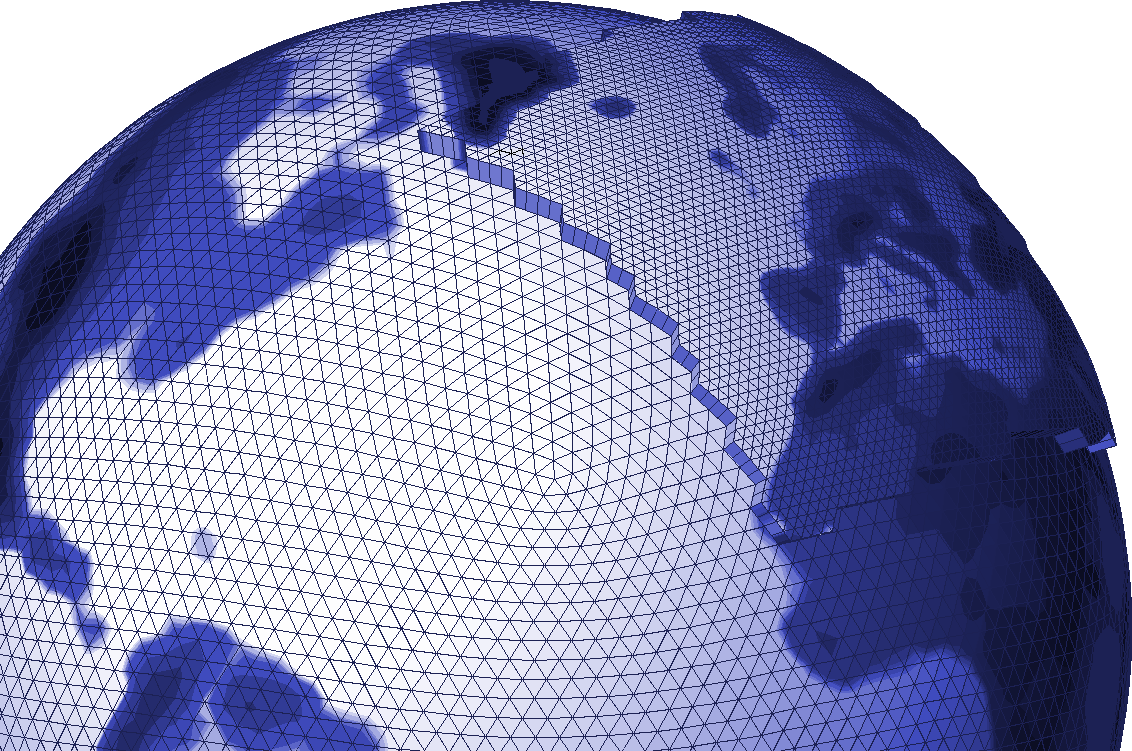
\includegraphics[width=0.75\textwidth]{icon_with_nest.png}
  \end{figure}
  \vspace{0.8cm}
  \textcolor{red}{\textbf{Version: \vhCurrentVersion}}\\
  \vspace{0.5cm}
  \textbf{Last changes: \today}\\
  \vspace{2.2cm}
  Offenbach am Main, Germany\\

  \newpage

\end{center}

\end{titlepage}
% ----------------------------------------------------------------%

\tableofcontents              %--- generate table of contents

% remove chapter number from header for abstracts
\renewcommand{\chaptermark}[1] {
  \markboth{#1}{}
}

% sign function
\newcommand{\sgn}{\operatorname{sgn}}


% use default again
\renewcommand{\chaptermark}[1]{%
  \markboth{\chaptername
    \ \thechapter.\ #1}{}}

\mainmatter                   %--- Zurcksetzen der Nummerierung auf arabisch


% ---------- Einbinden der verschiedenen Teildokumente -----------%
\svnInfo $Id$
\chapter{Available output fields in GRIB2-format}


In GRIB2, a variable is uniquely defined by the following set of metadata:
\begin{itemize}
 \item \emph{Discipline} (see GRIB2 code table 4.2)
 \item \emph{ParameterCategory} (see GRIB2 code table 4.2)
 \item \emph{ParameterNumber} (see GRIB2 code table 4.2)
 \item \emph{typeOfFirstfixedSurface} and \emph{typeOfSecondFixedSurface} (see GRIB2 code table 4.5)
 \item \emph{stepType} (instant, accum, avg, max, min, diff, rms, sd, cov, \dots)
\end{itemize}
A documentation of the official WMO GRIB2 code tables can be found here: \url{http://www.wmo.int/pages/prog/www/WMOCodes/WMO306_vI2/LatestVERSION/WMO306_vI2_GRIB2_CodeFlag_en.pdf}\\
In the following, \emph{typeOfFirstFixedSurface} and \emph{typeOfSecondFixedSurface} will be abbreviated by \emph{Lev-Typ~1/2}.



\section{Deprecated output fields}
With the launch of ICON, the following former GME output fields will no longer be available:

\begin{itemize}
 \item \textbf{BAS\_CON} [\textendash]: Level index of convective cloud base. Instead, \textbf{HBAS\_CON} [m] should be used.
 \item \textbf{TOP\_CON} [\textendash]: Level index of convective cloud top. Instead, \textbf{HTOP\_CON} [m] should be used.
 \item \textbf{T\_S} [K]: Temperature at the soil-atmosphere-, or soil-snow-interface. Note that $\mathrm{T\_S} = \mathrm{T\_SO(0)}$, thus $\mathrm{T\_S}$ is redundant.
 \item \textbf{W\_G1}, \textbf{W\_G2}  [mm H2O]: Soil water content in upper layer ($0$ to $10\,\mathrm{cm}$) and middle layer ($10$ to $100\,\mathrm{cm}$), respectively. 
                                                 If needed, these fields can be derived from \textbf{W\_SO}.
 \item \textbf{FIS} [$\mathrm{m^{2}\,s^{-1}}$]: Surface Geopotential. Instead, \textbf{HSURF} $[\mathrm{m}]$ should be used (see Section \ref{sec_newout}).
 \item \textbf{O3} [$\mathrm{kg/kg}$], \textbf{TO3} [$\mathrm{Dobson}$]: Ozone mixing ratio and corresponding total ozone concentration. No longer available; no substitution
\end{itemize}



\section{New output fields}\label{sec_newout}
Table \ref{table_newout} contains a list of new output fields that will become available with the launch of ICON (compared to GME). A more thorough description of these 
fields is provided in Section \ref{sec_outfields}.
\begin{table}[H]
\centering
\caption{Newly available output fields}\label{table_newout}
 \begin{tabular}{p{2.5cm}p{1.8cm}p{10.0cm}}
  \toprule
\multicolumn{1}{c}{\textbf{ShortName}}  &  \bf{Unit}                  & \multicolumn{1}{c}{\textbf{Description}}\\
\midrule
\textbf{W}                              &  $\mathrm{m/s}$             &  vertical velocity in height coordinates $w=\frac{\mathrm{d}z}{\mathrm{d}t}$ (3D field)\\
\textbf{DEN}                            &  $\mathrm{kg/m^{3}}$        &  density of moist air (3D field) \\
\textbf{TKE}                            &  $\mathrm{m^{2}/s^{2}}$     &  Turbulent kinetic energy (3D field) \\
\textbf{DTKE\_CON}                      &  $\mathrm{m^{2}/s^{3}}$     &  Buoyancy-production of TKE due to sub grid scale convection (3D field) \\
\textbf{HSURF}                          &  $\mathrm{m}$               &  Geometric Height of the earths surface above sea level (2D field) \\
\textbf{HHL}                            &  $\mathrm{m}$               &  Geometric Height of model half levels above sea level (3D field) \\
\textbf{CLON,CLAT}                      &  $\mathrm{deg}$             &  Geographical longitude/latitude of native grid triangle cell center \\
\textbf{ELON,ELAT}                      &  $\mathrm{deg}$             &  Geographical longitude/latitude of native grid triangle edge midpoint \\
\textbf{VLON,VLAT}                      &  $\mathrm{deg}$             &  Geographical longitude/latitude of native grid triangle vertex \\
  \bottomrule
 \end{tabular}
\end{table}




\section{Available output fields}\label{sec_outfields}

ICON output is available on two distinct horizontal grids: The native triangular grid with an average resolution of $13\,\mathrm{km}$, 
and a regular latitude-longitude grid with a resolution of $\Delta \lambda = \Delta \Phi=0.25^{\circ}$. On the native grid most output 
fields are defined on triangle cell centers, except for \texttt{VN}, which is defined on cell edges. On the lat-lon grid, all fields are 
defined on cell centers. A single 2D GRIB2 field on the native and regular lat-lon grid contains $2949120$ and $1036800$ grid points, respectively. 

For details regarding the available fields, please see the tables below. Note that the vertical rules in the leftmost column indicate, whether the field is 
available on the native grid ($\,$\markRed$\,$), on the lat-lon grid($\,$\markBlue$\,$), or on both grids($\,$\markRed\markBlue$\,$). 


\subsection{Time-constant (external parameter) fields}

Table \ref{table_constdb} provides an overview of the available time invariant fields. All except for \texttt{HHL}, \texttt{ELON}, \texttt{ELAT}, 
\texttt{VLON}, \texttt{VLAT} are available from the database category \texttt{CAT\_NAME=\$model\_\tblu{const}\_\tblu{an}\_\$suite}. See Section 
\ref{sec_skycat} for more details on the database categories and Section \ref{sec_example} for sample retrievals.

\begin{longtable}{@{}p{0.30cm}@{\hskip 0.05in}p{2.0cm}p{5.0cm}p{0.7cm}p{0.7cm}p{0.7cm}p{1.4cm}p{1cm}p{1cm}}
 \caption{Time-constant fields}\label{table_constdb}\\
  \toprule
&\multicolumn{1}{c}{\begin{sideways}\textbf{ShortName}\end{sideways}}  &  \multicolumn{1}{c}{\rb{\textbf{Description}}}  & \begin{sideways}\textbf{Discipline}\end{sideways} & \begin{sideways}\bf{Category}\end{sideways} & \begin{sideways}\bf{Number}\end{sideways}  & \begin{sideways}\bf{Lev-Typ 1/2}\end{sideways}  & \begin{sideways}\bf{stepType}\end{sideways} &\begin{sideways}\bf{Unit}\end{sideways}\\
\midrule
\endfirsthead
\caption[]{\emph{continued}}\\
\midrule
\endhead
\hline \multicolumn{8}{r}{\textit{Continued on next page}} \\
\endfoot
\endlastfoot
\multicolumn{8}{c}{\textbf{Date/Time} (YYYY-MM-DDThh) \textbf{D=0001-01-01T00}}\\
\midrule
\groups[tri][] & HSURF                         &  Geometric height of the earths surface above msl                                       &               0                                   &                       3                     &                    6                       &                 1/101                           &                      inst                   &        $\mathrm{m}$   \\
\groups[tri][] & HHL                           &  Geometric height of model half levels above msl                                        &               0                                   &                       3                     &                    6                       &                 150/101                         &                      inst                   &        $\mathrm{m}$   \\
\groups[tri][] & CLAT                          &  Geographical latitude of native grid triangle cell center                              &               0                                   &                     191                     &                    1                       &                 1/--                            &                      inst                   &        $\mathrm{Deg.\, N}$   \\
\groups[tri][] & CLON                          &  Geographical longitude of native grid triangle cell center                             &               0                                   &                     191                     &                    2                       &                 1/--                            &                      inst                   &        $\mathrm{Deg.\, E}$   \\
\groups[tri][] & ELAT                          &  Geographical latitude of native grid triangle edge midpoint                            &               0                                   &                     191                     &                    1                       &                 1/--                            &                      inst                   &        $\mathrm{Deg.\, N}$   \\
\groups[tri][] & ELON                          &  Geographical longitude of native grid triangle edge midpoint                           &               0                                   &                     191                     &                    2                       &                 1/--                            &                      inst                   &        $\mathrm{Deg.\, E}$   \\
\groups[tri][] & VLAT                          &  Geographical latitude of native grid triangle vertex                                   &               0                                   &                     191                     &                    1                       &                 1/--                            &                      inst                   &        $\mathrm{Deg.\, N}$   \\
\groups[tri][] & VLON                          &  Geographical longitude of native grid triangle vertex                                  &               0                                   &                     191                     &                    2                       &                 1/--                            &                      inst                   &        $\mathrm{Deg.\, E}$   \\
\groups[tri][] & FOR\_E                        &  Fraction of evergreen forest (possible range [$0,1$])                                  &               2                                   &                       0                     &                   29                       &                 1/--                            &                      inst                   &        $1$ \\
\groups[tri][] & FOR\_D                        &  Fraction of deciduous forest (possible range [$0,1$])                                  &               2                                   &                       0                     &                   30                       &                 1/--                            &                      inst                   &        $1$ \\
\groups[tri][] & FR\_LAND                      &  Land fraction (possible range [$0,1$])                                                 &               2                                   &                       0                     &                    0                       &                 1/--                            &                      inst                   &        $1$ \\
\groups[tri][] & FR\_LAKE                      &  Fresh water lake fraction (possible range [$0,1$])                                     &               1                                   &                       2                     &                    2                       &                 1/--                            &                      inst                   &        $1$ \\
\groups[tri][] & DEPTH\_LK                     &  Lake depth                                                                             &               1                                   &                       2                     &                    0                       &                 1/162                           &                      inst                   &        $\mathrm{m}$ \\
\groups[tri][] & ROOTDP                        &  Root depth of vegetation                                                               &               2                                   &                       0                     &                   32                       &                 1/--                            &                      inst                   &        $\mathrm{m}$ \\
\groups[tri][] & RSMIN                         &  Minimum stomatal resistance                                                            &               2                                   &                       0                     &                   16                       &                 1/--                            &                      inst                   &        $\mathrm{s\,m^{-1}}$ \\
\groups[tri][] & EMIS\_RAD                     &  Longwave surface emissivity                                                            &               2                                   &                       3                     &                  199                       &                 1/--                            &                      inst                   &        $1$ \\
\groups[tri][] & SOILTYP                       &  Soil type of land fraction  (9 types $[1,\dots, 9]$)                                   &               2                                   &                       3                     &                  196                       &                 1/--                            &                      inst                   &        $1$ \\
\groups[tri][] & SSO\_STDH                     &  Standard deviation of sub-grid scale orography                                         &               0                                   &                       3                     &                   20                       &                 1/--                            &                      inst                   &        $\mathrm{m}$ \\
\groups[tri][] & SSO\_GAMMA                    &  Anisotropy of sub-gridscale orography                                                  &               0                                   &                       3                     &                   24                       &                 1/--                            &                      inst                   &        $1$ \\
\groups[tri][] & SSO\_THETA                    &  Angle of sub-gridscale orography                                                       &               0                                   &                       3                     &                   21                       &                 1/--                            &                      inst                   &        $\mathrm{rad}$ \\
\groups[tri][] & SSO\_SIGMA                    &  Slope of sub-gridscale orography                                                       &               0                                   &                       3                     &                   22                       &                 1/--                            &                      inst                   &        $1$ \\
\groups[tri][] & LAI\_MX                       &  Leaf area index in the vegetation phase                                                &               2                                   &                       0                     &                   28                       &                 1/--                            &                      max                    &        $1$ \\
\groups[tri][] & NDVI\_MAX                     &  Normalized differential vegetation index                                               &               2                                   &                       0                     &                   31                       &                 1/--                            &                      max                    &        $1$ \\
\groups[tri][] & PLCOV\_MX                     &  Plant covering degree in the vegetation phase                                          &               2                                   &                       0                     &                    4                       &                 1/--                            &                      max                    &        $1$ \\
\groups[tri][] & T\_2M\_CL                     &  Climatological $2\,\mathrm{m}$ temperature (used as lower bc.\ for soil model)         &               0                                   &                       0                     &                    0                       &               103/--                            &                      inst                   &        $\mathrm{K}$ \\
\groups[tri][] & Z0                            &  Surface roughness length (over land)                                                   &               2                                   &                       0                     &                    1                       &                 1/--                            &                      inst                   &        $\mathrm{m}$ \\
\midrule
\multicolumn{8}{c}{\textbf{Date/Time} (YYYY-MM-DDThh) \textbf{D=1111-01-11T11}}\\
\midrule
\groups[tri][] & AER\_SS12                     &  Sea salt aerosol climatology (monthly fields)                                          &               0                                   &                      20                     &                   102                      &                 1/--                            &                      avg                    &        $\mathrm{1}$ \\
\groups[tri][] & AER\_DUST12                   &  Total soil dust aerosol climatology (monthly fields)                                   &               0                                   &                      20                     &                   102                      &                 1/--                            &                      avg                    &        $\mathrm{1}$ \\
\groups[tri][] & AER\_ORG12                    &  Organic aerosol climatology (monthly fields)                                           &               0                                   &                      20                     &                   102                      &                 1/--                            &                      avg                    &        $\mathrm{1}$ \\
\groups[tri][] & AER\_SO412                    &  Total sulfate aerosol climatology (monthly fields)                                     &               0                                   &                      20                     &                   102                      &                 1/--                            &                      avg                    &        $\mathrm{1}$ \\
\groups[tri][] & AER\_BC12                     &  Black carbon aerosol climatology (monthly fields)                                      &               0                                   &                      20                     &                   102                      &                 1/--                            &                      avg                    &        $\mathrm{1}$ \\
\groups[tri][] & ALB\_DIF12                    &  Shortwave ($0.3 - 5.0\,\mathrm{\mu m}$) albedo for diffuse radiation (monthly fields)  &               0                                   &                      19                     &                    18                      &                 1/--                            &                      avg                    &        $\mathrm{1}$ \\
\groups[tri][] & ALB\_UV12                     &  UV-visible ($0.3 - 0.7\,\mathrm{\mu m}$) albedo for diffuse radiation (monthly fields) &               0                                   &                      19                     &                   222                      &                 1/--                            &                      avg                    &        $\mathrm{1}$ \\
\groups[tri][] & ALB\_NI12                     &  Near infrared ($0.7 - 5.0\,\mathrm{\mu m}$) albedo for diffuse radiation (monthly fields) &            0                                   &                      19                     &                   223                      &                 1/--                            &                      avg                    &        $\mathrm{1}$ \\
\groups[tri][] & NDVI\_MRAT                    &  ratio of monthly mean NDVI (normalized differential vegetation index) to annual max    &               0                                   &                       0                     &                   192                      &                 1/--                            &                      avg                    &        $\mathrm{1}$ \\
  \bottomrule
\end{longtable}
%  \bottomrule
% \end{tabular}
%\end{table}



\subsection{Multi-level fields on native hybrid vertical levels}

\begin{table}[H]
\caption{Hybrid multi-level forecast ($VV>0$) and initialised analysis ($VV=0$) products}
 \begin{tabular}{@{}p{0.30cm}@{\hskip 0.05in}p{2.0cm}p{5.0cm}p{0.6cm}p{0.6cm}p{0.6cm}p{1.4cm}p{1cm}p{1cm}}
  \toprule
&\multicolumn{1}{c}{\begin{sideways}\textbf{ShortName}\end{sideways}}  &  \multicolumn{1}{c}{\rb{\textbf{Description}}}  & \begin{sideways}\textbf{Discipline}\end{sideways} & \begin{sideways}\bf{Category}\end{sideways} & \begin{sideways}\bf{Number}\end{sideways}  & \begin{sideways}\bf{Lev-Typ 1/2}\end{sideways}  & \begin{sideways}\bf{stepType}\end{sideways} &\begin{sideways}\bf{Unit}\end{sideways}\\
\midrule
\groups[tri][] & U                          &  Zonal wind                                                                                &               0                                   &                     2                       &                    2                       &                 150/150                         &                      inst                   &        $\mathrm{m\,s^{-1}}$   \\ 
\groups[tri][] & V                          &  Meridional wind                                                                           &               0                                   &                     2                       &                    3                       &                 150/150                         &                      inst                   &        $\mathrm{m\,s^{-1}}$   \\
\groups[tri][] & W                          &  Vertical wind                                                                             &               0                                   &                     2                       &                    9                       &                 150/--                          &                      inst                   &        $\mathrm{m\,s^{-1}}$   \\
\groups[tri][] & T                          &  Temperature                                                                               &               0                                   &                     0                       &                    0                       &                 150/150                         &                      inst                   &        $\mathrm{K}$          \\
\groups[tri][] & DEN                        &  Density of moist air                                                                      &               0                                   &                     3                       &                    10                      &                 150/150                         &                      inst                   &        $\mathrm{kg\,m^{-3}}$ \\
\groups[tri][] & QV                         &  Specific humidity                                                                         &               0                                   &                     1                       &                    0                       &                 150/150                         &                      inst                   &        $\mathrm{kg\,kg^{-1}}$ \\
\groups[tri][] & QC                         &  \textcolor{red}{Cloud mixing ratio}\footnotemark[2]                                       &               0                                   &                     1                       &                    22                      &                 150/150                         &                      inst                   &        $\mathrm{kg\,kg^{-1}}$ \\
\groups[tri][] & QI                         &  \textcolor{red}{Cloud ice mixing ratio}\footnotemark[2]                                   &               0                                   &                     1                       &                    82                      &                 150/150                         &                      inst                   &        $\mathrm{kg\,kg^{-1}}$ \\
\groups[tri][] & QR                         &  \textcolor{red}{Rain mixing ratio}\footnotemark[2]                                        &               0                                   &                     1                       &                    24                      &                 150/150                         &                      inst                   &        $\mathrm{kg\,kg^{-1}}$ \\
\groups[tri][] & QS                         &  \textcolor{red}{Snow mixing ratio}\footnotemark[2]                                        &               0                                   &                     1                       &                    25                      &                 150/150                         &                      inst                   &        $\mathrm{kg\,kg^{-1}}$ \\
\groups[tri][] & CLC                        &  Cloud cover                                                                               &               0                                   &                     6                       &                    22                      &                 150/150                         &                      inst                   &        $\mathrm{\%}$ \\
\groups[tri][] & TKE                        &  Turbulent kinetic energy                                                                  &               0                                   &                     19                      &                    11                      &                 150/--                          &                      inst                   &        $\mathrm{m^{2}\,s^{-2}}$ \\
\groups[tri][] & DTKE\_CON                  &  Buoyancy-production of TKE due to sub grid scale convection                               &               0                                   &                     19                      &                    219                     &                 150/--                          &                      inst                   &        $\mathrm{m^{2}\,s^{-3}}$ \\                                  
  \bottomrule
 \end{tabular}
\end{table}
\footnotetext[2]{for the time being, erroneously encoded as mixing ratios instead of specific quantities}




\subsection{Multi-level fields interpolated to pressure levels}

The following pressure levels are available: $1000$, $950$, $925$, $900$, $850$, $800$, $700$, $600$, $500$, $400$, $300$, $250$, $200$, $150$, $100$, 
$70$, $50$, $30$, \textcolor{red}{$20$}, $10$, \textcolor{red}{$7$}, $5$, \textcolor{red}{$3$}, \textcolor{red}{$2$}, \textcolor{red}{$1$}, 
\textcolor{red}{$0.3$}, \textcolor{red}{$0.1$} $\mathrm{hPa}$. Newly available 
pressure levels (as compared to GME) are highlighted in red. I.e.\ note that all $17$ WMO standard pressure levels are included.

\begin{table}[H]
\caption{Multi-level forecast ($VV>0$) and initialised analysis ($VV=0$) products interpolated to pressure levels}
 \begin{tabular}{@{}p{0.30cm}@{\hskip 0.05in}p{2.0cm}p{5.0cm}p{0.6cm}p{0.6cm}p{0.6cm}p{1.4cm}p{1cm}p{1cm}}
  \toprule
&\multicolumn{1}{c}{\begin{sideways}\textbf{ShortName}\end{sideways}}  &  \multicolumn{1}{c}{\rb{\textbf{Description}}}  & \begin{sideways}\textbf{Discipline}\end{sideways} & \begin{sideways}\bf{Category}\end{sideways} & \begin{sideways}\bf{Number}\end{sideways}  & \begin{sideways}\bf{Lev-Typ 1/2}\end{sideways}  & \begin{sideways}\bf{stepType}\end{sideways} &\begin{sideways}\bf{Unit}\end{sideways}\\
\midrule
\groups[][ll] & FI                         &  Geopotential                                                                              &               0                                   &                     3                       &                    4                       &                 100/--                          &                      inst                   &        $\mathrm{m^{2}\,s^{-2}}$   \\
\groups[][ll] & OMEGA                      &  Vertical velocity in pressure coordinates ($\omega=\mathrm{d}p/\mathrm{d}t$)              &               0                                   &                     2                       &                    8                       &                 100/--                          &                      inst                   &        $\mathrm{Pa\,s^{-1}}$  \\
\groups[][ll] & RELHUM                     &  Relative humidity (with respect to water)                                                 &               0                                   &                     1                       &                    1                       &                 100/--                          &                      inst                   &        $\mathrm{\%}$          \\
\groups[][ll] & T                          &  Temperature                                                                               &               0                                   &                     0                       &                    0                       &                 100/--                          &                      inst                   &        $\mathrm{K}$          \\
\groups[][ll] & U                          &  Zonal wind                                                                                &               0                                   &                     2                       &                    2                       &                 100/--                          &                      inst                   &        $\mathrm{m\,s^{-1}}$   \\ 
\groups[][ll] & V                          &  Meridional wind                                                                           &               0                                   &                     2                       &                    3                       &                 100/--                          &                      inst                   &        $\mathrm{m\,s^{-1}}$   \\
  \bottomrule
 \end{tabular}
\end{table}




\subsection{Single-level fields}

\begin{longtable}{@{}p{0.30cm}@{\hskip 0.05in}p{2.0cm}p{5.0cm}p{0.7cm}p{0.7cm}p{0.7cm}p{1.4cm}p{1cm}p{1cm}}
\caption[]{Single-level forecast ($VV>0$) and initialised analysis ($VV=0$) products}\\
  \toprule
&\multicolumn{1}{c}{\begin{sideways}\textbf{ShortName}\end{sideways}}  &  \multicolumn{1}{c}{\rb{\textbf{Description}}}  & \begin{sideways}\textbf{Discipline}\end{sideways} & \begin{sideways}\bf{Category}\end{sideways} & \begin{sideways}\bf{Number}\end{sideways}  & \begin{sideways}\bf{Lev-Typ 1/2}\end{sideways}  & \begin{sideways}\bf{stepType}\end{sideways} &\begin{sideways}\bf{Unit}\end{sideways}\\
\midrule
\endfirsthead
\caption[]{\emph{continued}}\\
\midrule
\endhead
\hline \multicolumn{8}{r}{\textit{Continued on next page}} \\
\endfoot
\endlastfoot
\groups[tri][ll] & PS                             &  Surface pressure (not reduced)                                                        &               0                                   &                     3                       &                    0                       &                 1/--                            &                      inst                   &        $\mathrm{Pa}$   \\ 
\groups[tri][ll] & T\_SNOW                        &  Temperature of the snow surface                                                       &               0                                   &                     0                       &                    18                      &                 1/--                            &                      inst                   &        $\mathrm{K}$    \\
\groups[tri][ll] & T\_G                           &  Ground temperature (temperature at sfc-atm interface)                                 &               0                                   &                     0                       &                    0                       &                 1/--                            &                      inst                   &        $\mathrm{K}$    \\
\groups[tri][ll] & QV\_S                          &  Surface specific humidity                                                             &               0                                   &                     1                       &                    0                       &                 1/--                            &                      inst                   &        $\mathrm{kg\,kg^{-1}}$    \\
\groups[tri][ll] & W\_SNOW                        &  Snow depth water equivalent                                                           &               0                                   &                     1                       &                    60                      &                 1/--                            &                      inst                   &        $\mathrm{kg\,m^{-2}}$    \\
\groups[tri][]   & W\_I                           &  Plant canopy surface water                                                            &               2                                   &                     0                       &                    13                      &                 1/--                            &                      inst                   &        $\mathrm{kg\,m^{-2}}$    \\
\groups[tri][]   & TCM                            &  Turbulent transfer coefficient for momentum (surface)                                 &               0                                   &                     2                       &                    29                      &                 1/--                            &                      inst                   &        $1$    \\ 
\groups[tri][]   & TCH                            &  Turbulent transfer coefficient for heat and moisture (surface)                        &               0                                   &                     0                       &                    19                      &                 1/--                            &                      inst                   &        $1$    \\
\groups[tri][ll] & ASOB\_S                        &  Net short-wave radiation flux at surface (average since model start)                  &               0                                   &                     4                       &                     9                      &                 1/--                            &                      avg                    &        $\mathrm{W\,m^{-2}}$    \\
\groups[tri][ll] & ATHB\_S                        &  Net long-wave radiation flux at surface (average since model start)                   &               0                                   &                     5                       &                     5                      &                 1/--                            &                      avg                    &        $\mathrm{W\,m^{-2}}$    \\
\groups[][ll]    & APAB\_S                        &  Photosynthetically active radiation flux at surface (average since model start)       &               0                                   &                     4                       &                    10                      &                 1/--                            &                      avg                    &        $\mathrm{W\,m^{-2}}$    \\
\groups[tri][ll] & ASOB\_T                        &  Net short-wave radiation flux at TOA (average since model start)                      &               0                                   &                     4                       &                     9                      &                 8/--                            &                      avg                    &        $\mathrm{W\,m^{-2}}$    \\
\groups[tri][ll] & ATHB\_T                        &  Net long-wave radiation flux at TOA (average since model start)                       &               0                                   &                     5                       &                     5                      &                 8/--                            &                      avg                    &        $\mathrm{W\,m^{-2}}$    \\ 
\groups[tri][ll] & ASWDIR\_S                      &  Surface down solar direct radiation (average since model start)                       &               0                                   &                     4                       &                   198                      &                 1/--                            &                      avg                    &        $\mathrm{W\,m^{-2}}$  \\
\groups[tri][ll] & ASWDIFD\_S                     &  Surface down solar diffuse radiation (average since model start)                      &               0                                   &                     4                       &                   199                      &                 1/--                            &                      avg                    &        $\mathrm{W\,m^{-2}}$  \\
\groups[tri][ll] & ASWDIFU\_S                     &  Surface up solar diffuse radiation (average since model start)                        &               0                                   &                     4                       &                     8                      &                 1/--                            &                      avg                    &        $\mathrm{W\,m^{-2}}$  \\
\groups[tri][ll] & ALB\_RAD                       &  Surface albedo for visible range, diffuse                                             &               0                                   &                    19                       &                     1                      &                 1/--                            &                      inst                   &        $\mathrm{\%}$    \\
\groups[tri][ll] & RAIN\_GSP\footnotemark[4]      &  Large scale rain (accumulated since model start)                                      &               0                                   &                     1                       &                    77                      &                 1/--                            &                      accu                   &        $\mathrm{kg\,m^{-2}}$    \\
\groups[tri][ll] & SNOW\_GSP\footnotemark[4]      &  Large snowfall water equivalent (accumulated since model start)                       &               0                                   &                     1                       &                    56                      &                 1/--                            &                      accu                   &        $\mathrm{kg\,m^{-2}}$    \\
\groups[tri][ll] & RAIN\_CON\footnotemark[4]      &  Convective rain (accumulated since model start)                                       &               0                                   &                     1                       &                    76                      &                 1/--                            &                      accu                   &        $\mathrm{kg\,m^{-2}}$    \\
\groups[tri][ll] & SNOW\_CON\footnotemark[4]      &  Convective snowfall water equivalent (accumulated since model start)                  &               0                                   &                     1                       &                    55                      &                 1/--                            &                      accu                   &        $\mathrm{kg\,m^{-2}}$    \\
\groups[tri][ll] & TOT\_PREC\footnotemark[4]      &  Total precipitation (accumulated since model start)                                   &               0                                   &                     1                       &                    52                      &                 1/--                            &                      accu                   &        $\mathrm{kg\,m^{-2}}$  \\
\groups[tri][ll] & RUNOFF\_S                      &  Surface water runoff (accumulated since model start)                                  &               2                                   &                     0                       &                     5                      &                 106/--                          &                      accu                   &        $\mathrm{kg\,m^{-2}}$  \\
\groups[tri][ll] & RUNOFF\_G                      &  Soil water runoff (accumulated since model start)                                     &               2                                   &                     0                       &                     5                      &                 106/--                          &                      accu                   &        $\mathrm{kg\,m^{-2}}$  \\                                      
\groups[tri][ll] & U\_10M                         &  Zonal wind at 10m above ground                                                        &               0                                   &                     2                       &                     2                      &               103/--                            &                      inst                   &        $\mathrm{m\,s^{-1}}$  \\
\groups[tri][ll] & V\_10M                         &  Meridional wind at 10m above ground                                                   &               0                                   &                     2                       &                     3                      &               103/--                            &                      inst                   &        $\mathrm{m\,s^{-1}}$  \\
\groups[tri][ll] & T\_2M                          &  Temperature at 2m above ground                                                        &               0                                   &                     0                       &                     0                      &               103/--                            &                      inst                   &        $\mathrm{K}$          \\
\groups[tri][ll] & TD\_2M                         &  Dew point temperature at 2m above ground                                              &               0                                   &                     0                       &                     6                      &               103/--                            &                      inst                   &        $\mathrm{K}$          \\
\groups[tri][ll] & TMAX\_2M                       &  Maximum temperature at 2m above ground                                                &               0                                   &                     0                       &                     0                      &               103/--                            &                      max                    &        $\mathrm{K}$          \\
\groups[tri][ll] & TMIN\_2M                       &  Minimum temperature at 2m above ground                                                &               0                                   &                     0                       &                     0                      &               103/--                            &                      min                    &        $\mathrm{K}$          \\
\groups[tri][ll] & VMAX\_10M                      &  Maximum wind at $10\,\mathrm{m}$ above ground                                         &               0                                   &                     2                       &                    22                      &               103/--                            &                      max                    &        $\mathrm{m\,s^{-1}}$   \\
\groups[tri][ll] & Z0                             &  Surface roughness (above land and water)                                              &               2                                   &                     0                       &                     1                      &                 1/--                            &                      inst                   &        $\mathrm{m}$          \\
\groups[tri][ll] & CLCT                           &  Total cloud cover                                                                     &               0                                   &                     6                       &                     1                      &                 1/--                            &                      inst                   &        $\mathrm{\%}$          \\
\groups[tri][ll] & CLCT\_MOD                      &  Modified total cloud cover for media                                                  &               0                                   &                     6                       &                   199                      &                 1/--                            &                      inst                   &        $1$                    \\
\groups[tri][ll] & CLDEPTH                        &  Modified cloud depth for media                                                        &               0                                   &                     6                       &                   198                      &                 1/--                            &                      inst                   &        $1$                    \\
\groups[tri][ll] & CLCH                           &  High level clouds                                                                     &               0                                   &                     6                       &                    22                      &                 100/100                         &                      inst                   &        $\mathrm{\%}$          \\
\groups[tri][ll] & CLCM                           &  Mid level clouds                                                                      &               0                                   &                     6                       &                    22                      &                 100/100                         &                      inst                   &        $\mathrm{\%}$          \\
\groups[tri][ll] & CLCL                           &  Low level clouds                                                                      &               0                                   &                     6                       &                    22                      &                 100/1                           &                      inst                   &        $\mathrm{\%}$          \\
\groups[tri][ll] & TQV                            &  Column integrated water vapour (grid scale)                                           &               0                                   &                     1                       &                    64                      &                 1/--                            &                      inst                   &        $\mathrm{kg\,m^{-2}}$  \\
\groups[tri][ll] & TQC                            &  Column integrated cloud water (grid scale)                                            &               0                                   &                     1                       &                    69                      &                 1/--                            &                      inst                   &        $\mathrm{kg\,m^{-2}}$  \\
\groups[tri][ll] & TQI                            &  Column integrated cloud ice (grid scale)                                              &               0                                   &                     1                       &                    70                      &                 1/--                            &                      inst                   &        $\mathrm{kg\,m^{-2}}$  \\
\groups[tri][ll] & TQR                            &  Column integrated rain (grid scale)                                                   &               0                                   &                     1                       &                    45                      &                 1/--                            &                      inst                   &        $\mathrm{kg\,m^{-2}}$  \\
\groups[tri][ll] & TQS                            &  Column integrated snow (grid scale)                                                   &               0                                   &                     1                       &                    46                      &                 1/--                            &                      inst                   &        $\mathrm{kg\,m^{-2}}$  \\
\groups[tri][ll] & TQC\_DIA                       &  Total column integrated cloud water (including sub-grid-scale contribution)           &               0                                   &                     1                       &                   215                      &                 1/--                            &                      inst                   &        $\mathrm{kg\,m^{-2}}$  \\
\groups[tri][ll] & TQI\_DIA                       &  Total column integrated cloud ice (including sub-grid-scale contribution)             &               0                                   &                     1                       &                   216                      &                 1/--                            &                      inst                   &        $\mathrm{kg\,m^{-2}}$  \\
\groups[tri][ll] & HBAS\_CON                      &  Height of convective cloud base above msl                                             &               0                                   &                     6                       &                    26                      &                 2/101                           &                      inst                   &        $\mathrm{m}$  \\
\groups[tri][ll] & HTOP\_CON                      &  Height of convective cloud top above msl                                              &               0                                   &                     6                       &                    27                      &                 3/101                           &                      inst                   &        $\mathrm{m}$  \\
\groups[tri][ll] & HTOP\_DC                       &  Height of top of dry convection above msl                                             &               0                                   &                     6                       &                   196                      &                 3/101                           &                      inst                   &        $\mathrm{m}$  \\
\groups[tri][ll] & HZEROCL                        &  Height of 0 degree Celsius isotherm above msl                                         &               0                                   &                     3                       &                     6                      &                 4/101                           &                      inst                   &        $\mathrm{m}$  \\
\groups[tri][ll] & AUMFL\_S                       &  U-momentum flux at surface $\overline{u^{\prime}w^{\prime}}^{1/2}$ (average since model start)&       0                                   &                     2                       &                    17                      &                 1/--                            &                      avg                    &        $\mathrm{m}$  \\
\groups[tri][ll] & AVMFL\_S                       &  V-momentum flux at surface $\overline{v^{\prime}w^{\prime}}^{1/2}$ (average since model start)&       0                                   &                     2                       &                    18                      &                 1/--                            &                      avg                    &        $\mathrm{m}$  \\
\groups[tri][ll] & ASHFL\_S                       &  Sensible heat net flux at surface (average since model start)                         &               0                                   &                     0                       &                    11                      &                 1/--                            &                      avg                    &        $\mathrm{W\,m^{-2}}$  \\
\groups[tri][ll] & ALHFL\_S                       &  Latent heat net flux at surface (average since model start)                           &               0                                   &                     0                       &                    10                      &                 1/--                            &                      avg                    &        $\mathrm{W\,m^{-2}}$  \\
\groups[tri][ll] & FR\_ICE                        &  Sea/lake ice cover  (possible range: $[0,1]$)                                         &              10                                   &                     2                       &                     0                      &                 1/--                            &                      inst                   &        $1$  \\
\groups[tri][ll] & T\_ICE                         &  Sea ice temperature (at ice-atm interface)                                            &              10                                   &                     2                       &                     8                      &                 1/--                            &                      inst                   &        $\mathrm{K}$  \\
\groups[tri][ll] & H\_ICE                         &  Sea ice thickness (Max: $3\,\mathrm{m}$)                                              &              10                                   &                     2                       &                     1                      &                 1/--                            &                      inst                   &        $\mathrm{m}$  \\
\groups[tri][]   & FRESHSNW                       &  Fresh snow factor (weighting function for albedo indicating freshness of snow)        &               0                                   &                     1                       &                   203                      &                 1/--                            &                      inst                   &        $1$  \\
\groups[tri][ll] & RHO\_SNOW                      &  Snow density                                                                          &               0                                   &                     1                       &                    61                      &                 1/--                            &                      inst                   &        $\mathrm{kg\,m^{-3}}$  \\
\groups[tri][ll] & H\_SNOW                        &  Snow depth                                                                            &               0                                   &                     1                       &                    11                      &                 1/--                            &                      inst                   &        $\mathrm{m}$  \\
\groups[tri][]   & PLCOV                          &  Plant cover                                                                           &               2                                   &                     0                       &                     4                      &                 1/--                            &                      inst                   &        $\mathrm{\%}$ \\
\groups[tri][]   & LAI                            &  Leaf area index                                                                       &               2                                   &                     0                       &                    28                      &                 1/--                            &                      inst                   &        $1$ \\
\groups[tri][]   & NDVIRATIO                      &  ratio of current NDVI (normalized differential vegetation index) to annual max        &               2                                   &                     0                       &                   192                      &                 1/--                            &                      inst                   &        $1$ \\
\groups[tri][ll] & WW                             &  Weather interpretation  (WMO)                                                         &               0                                   &                    19                       &                    25                      &                 1/--                            &                      inst                   &        $1$ \\
  \bottomrule
\end{longtable}



\footnotetext[4]{Note that the unit which is displayed, when inspecting the GRIB2 message with \emph{grib\_dump} is $\mathrm{kg\,m^{-2}\,s^{-1}}$ 
rather than $\mathrm{kg\,m^{-2}}$. Mathematically this is wrong, however, it is in accordance with the GRIB2 standard. To get the mathematically correct 
unit for accumulated fields (\emph{typeOfStatisticalProcessing}=1), the unit displayed by \emph{grib\_dump} must be multiplied by $\mathrm{s}$.}


\begin{longtable}{@{}p{0.30cm}@{\hskip 0.05in}p{2.0cm}p{5.0cm}p{0.6cm}p{0.6cm}p{0.6cm}p{1.4cm}p{1cm}p{1cm}}
\caption[]{Multi-level forecast ($VV>0$) and initialised analysis ($VV=0$) products of the soil model}\\
  \toprule
&\multicolumn{1}{c}{\begin{sideways}\textbf{ShortName}\end{sideways}}  &  \multicolumn{1}{c}{\rb{\textbf{Description}}}  & \begin{sideways}\textbf{Discipline}\end{sideways} & \begin{sideways}\bf{Category}\end{sideways} & \begin{sideways}\bf{Number}\end{sideways}  & \begin{sideways}\bf{Lev-Typ 1/2}\end{sideways}  & \begin{sideways}\bf{stepType}\end{sideways} &\begin{sideways}\bf{Unit}\end{sideways}\\
\midrule
%\endfirsthead
%\caption[]{\emph{continued}}\\
%\midrule
\endhead
\hline \multicolumn{8}{r}{\textit{Continued on next page}} \\
\endfoot
\endlastfoot
\groups[tri][ll] & T\_SO                          &  Soil temperature                                                                      &               2                                   &                     3                       &                    18                       &               106/--                           &                      inst                   &        $\mathrm{K}$   \\
\groups[tri][ll] & W\_SO                          &  Soil moisture integrated over individual soil layers  (ice + liquid)                  &               2                                   &                     3                       &                    20                       &               106/106                          &                      inst                   &        $\mathrm{kg\,m^{-2}}$   \\
\groups[tri][ll] & W\_SO\_ICE                     &  Soil ice content integrated over individual soil layers                               &               2                                   &                     3                       &                    22                       &               106/106                          &                      inst                   &        $\mathrm{kg\,m^{-2}}$   \\
  \bottomrule
\end{longtable}

Soil temperature is defined at the soil depths given in Table \ref{tab_soillayer} (column 2). Levels $1$ to $8$ define the full levels of the soil model. A zero gradient 
condition is assumed between levels $0$ and $1$, meaning that temperatures at the surface-atmosphere interface are set equal to the temperature at the first full level depth.
($0.5\,\mathrm{cm}$). Temperatures are prognosed for layers $1$ to $7$. At the lowermost layer (mid-level height $1458\,\mathrm{cm}$) the temperature is fixed 
to the climatological average $2\,\mathrm{m}$-temperature.

Soil moisture \texttt{W\_SO} is prognosed for layers $1$ to $6$. In the two lowermost layers \texttt{W\_SO} is filled with \texttt{W\_SO(6)} (zero gradient condition).

\begin{table}
\center
\caption{Soil model: vertical distribution of levels and layers}\label{tab_soillayer}
 \begin{tabular}{>{\centering\arraybackslash}p{2.0cm}>{\centering\arraybackslash}p{2.5cm}|>{\centering\arraybackslash}p{2.5cm}>{\centering\arraybackslash}p{5.0cm}}
 \toprule
  \bf{level no.}       &  \bf{depth [cm]}        &   \bf{layer no.}        & \bf{upper/lower bounds [cm]} \\
 \midrule
         0             &     $0.0$               &                         &                                     \\
         1             &     $0.5$               &         1               &     $0.0$\, \textemdash\, $1.0$     \\
         2             &     $2.0$               &         2               &     $1.0$\, \textemdash\, $3.0$     \\
         3             &     $6.0$               &         3               &     $3.0$\, \textemdash\, $9.0$     \\
         4             &     $18.0$              &         4               &     $9.0$\, \textemdash\, $27.0$    \\
         5             &     $54.0$              &         5               &    $27.0$\, \textemdash\, $81.0$    \\
         6             &     $162.0$             &         6               &    $81.0$\, \textemdash\, $243.0$   \\
         7             &     $486.0$             &         7               &   $243.0$\, \textemdash\, $729.0$   \\
         8             &     $1458.0$            &         8               &   $729.0$\, \textemdash\, $2187.0$  \\
 \bottomrule
 \end{tabular}
\end{table}



\subsection{Surface fields interpolated to msl}
\begin{table}[H]
\caption{Forecast ($VV>0$) and initialised analysis ($VV=0$) products interpolated to msl}
 \begin{tabular}{@{}p{0.30cm}@{\hskip 0.05in}p{2.0cm}p{5.0cm}p{0.7cm}p{0.7cm}p{0.7cm}p{1.4cm}p{1cm}p{1cm}}
  \toprule
&\multicolumn{1}{c}{\begin{sideways}\textbf{ShortName}\end{sideways}}  &  \multicolumn{1}{c}{\rb{\textbf{Description}}}  & \begin{sideways}\textbf{Discipline}\end{sideways} & \begin{sideways}\bf{Category}\end{sideways} & \begin{sideways}\bf{Number}\end{sideways}  & \begin{sideways}\bf{Lev-Typ 1/2}\end{sideways}  & \begin{sideways}\bf{stepType}\end{sideways} &\begin{sideways}\bf{Unit}\end{sideways}\\
\midrule
\groups[][ll] & PMSL                       &  Surface pressure reduced to msl                                                           &               0                                   &                     3                       &                    1                       &                 101/--                          &                      inst                   &        $\mathrm{Pa}$   \\
  \bottomrule
 \end{tabular}
\end{table}


\section{Extended description of available output fields}

In order to facilitate the selection and interpretation of fields and to guard against possible mis-interpretation or mis-usage, the following section provides a more thorough 
description of the available output fields.

%\subsection{External parameter}

% uses package enumitem
%\begin{description}[font=\sffamily\bfseries, leftmargin=3.0cm,style=sameline]
%\begin{description}[leftmargin=3.0cm,style=sameline]
% \item [AER\_SS] description of Hello
% \item [AER\_DUST12] another description
%\end{description}


\subsection{Cloud products}
% uses package enumitem
%\begin{description}[font=\sffamily\bfseries, leftmargin=3.0cm,style=sameline]
\begin{description}[leftmargin=3.0cm,style=sameline]
  \item [CLCT\_MOD] Modified total cloud cover ($0 \leq$ \texttt{CLCT\_MOD} $\leq 1$). Used for visualization purpose 
                    (i.e.\ gray-scale figures) in the media. It is derived from \texttt{CLC}, neglecting cirrus clouds if 
                    there are only high clouds present at a given grid point. The reason for this treatment is that 
                    the general public does not regard transparent cirrus clouds as `real' clouds.
  \item [CLDEPTH]   Modified cloud depth ($0 \leq$ \texttt{CLDEPTH} $\leq 1$). Used for visualization purpose (i.e.\ gray-scale figures) 
                    in the media. A cloud reaching a vertical extent of $700\,\mathrm{hPa}$ or more, has \texttt{CLDEPTH}= $1$.
  \item [HBAS\_CON] Height of the convective cloud base in m above msl. \texttt{HBAS\_CON} is initialized with $-500\,\mathrm{m}$ 
                    at points where no convection is diagnosed.
  \item [HTOP\_CON] Same, but for cloud top.
\end{description}


\subsection{Near surface products}
% uses package enumitem
%\begin{description}[font=\sffamily\bfseries, leftmargin=3.0cm,style=sameline]
\begin{description}[leftmargin=3.0cm,style=sameline]
  \item [TMIN\_2M]  Minimum temperature at $2\,\mathrm{m}$ above ground, computed over $3$-hourly intervals. 
  \item [TMAX\_2M]  Same, but for maximum $2\,\mathrm{m}$ temperature.
  \item [VMAX\_10M] Maximum wind gust at $10\,\mathrm{m}$ above ground, computed over $3$-hourly intervals. It is diagnosed 
                    from the turbulence state in the atmospheric boundary layer, including a potential enhancement by the 
                    SSO parameterization over mountainous terrain. In the presence of deep convection, it contains an additional 
                    contribution due to convective gusts.
\end{description}



\subsubsection{General comment on statistically processed fields}

In GRIB2, the overall time interval over which a statistical process (like averaging, computation of maximum/minimum) has taken place is 
encoded as follows:

The beginning of the overall time interval is defined by \texttt{referenceTime + forecastTime}, whereas the end of the 
overall time interval is given by \texttt{referenceTime + forecastTime + lengthOfTimeRange}.

%\begin{note}%
%\textbf{Note:} Fields for which the beginning of the time interval differs from \texttt{referenceTime} are currently 
%encoded incorrectly. The begining of the time interval is erroneously set to \texttt{referenceTime}. I.e.\ this is currently the case 
%for \texttt{TMAX\_2M}, \texttt{TMIN\_2M}, \texttt{VMAX\_10M}.
%\end{note}

%\subsection{Atmospheric products}


\subsection{Surface products}
% uses package enumitem
%\begin{description}[font=\sffamily\bfseries, leftmargin=3.0cm,style=sameline]
\begin{description}[leftmargin=3.0cm,style=sameline]
% \item [APAB\_S] Photosynthetically active radiation flux at the surface, i.e.\ that part of the net short-wave radiation flux 
%                 that photosynthetic organisms are able to use in the process of photosynthesis. This is approximately the case for 
%                 solar radiation in the spectrakl range from $400$ to $700\,\mathrm{nm}$. Average over forecast time.

 \item [FR\_ICE] Sea and lake ice cover. Currently, the only possible values are $0$ (no ice cover) and $1$ (ice covered grid point). For 
                 lake points, \texttt{FR\_ICE} is synchronized with \texttt{H\_ICE} meaning that \texttt{FR\_ICE} is set to $1$ ($0$), 
                 where the lake model indicates $\texttt{H\_ICE}>0$ ($\texttt{H\_ICE}=0$).

 \item [H\_ICE] Ice thickness over sea and frozen fresh water lakes. The maximum allowable ice thickness is limited to $3\,\mathrm{m}$. 
                New sea-ice points generated by the analysis are initialized with $\texttt{H\_ICE}=0.5\,\mathrm{m}$.

 \item [T\_ICE] Ice temperature over sea-ice and frozen lake points. Melting ice has a temperature of $273.15\,\mathrm{K}$. Ice-free 
                points over land, sea, and lakes are set to \texttt{T\_SO(0)}.

 \item [T\_G]   Temperature at the atmosphere-surface interface. It is the temperature that is crucial for the computation of surface fluxes. 
                \texttt{T\_G} is equal to \texttt{T\_SO(0)} over open water and snow-free land. At other grid points one has
                \begin{itemize} 
                  \item $\texttt{T\_G}=\texttt{T\_SNOW} + (1 - \mathrm{f\_snow})*(\texttt{T\_SO(0)} - \texttt{T\_SNOW})$ over (partially) 
                        snow covered grid points. $\mathrm{f\_snow}$ is the grid point fraction that is snow covered.
                  \item $\texttt{T\_G}=\texttt{T\_ICE}$ over frozen sea and fresh water lakes
                \end{itemize}

 \item [TOT\_PREC] Total precipitation accumulated since model start.\\
                \texttt{TOT\_PREC = RAIN\_GSP + SNOW\_GSP + RAIN\_CON + SNOW\_CON}
                
 \item [W\_I]   Water content of interception layer, i.e.\ the amount of precipitation intercepted by vegetation canopies. The maximum 
                capacity of the interception reservoir is currently limited to $6.0E-3\,\mathrm{kg\,m^{-2}}$ due to numerical reasons 
                and thus almost negligible. Over water points, \texttt{W\_I} is set to 0.

 \item [Z0]     Surface roughness length. Constant over land, where it depends only on the type of land cover. I.e.\ it does 
                not contain any contribution from subgrid-scale orography. Over water, the roughness length usually varies 
                with time. It is computed by the so called Charnock-formula, which parameterizes the impact of waves on the 
                roughness length. Note that this field differs significantly from the extermal parameter field \texttt{Z0} 
                (see Table \ref{table_extpar_products} or \ref{table_constdb}).  
\end{description}


\subsection{Soil products}
% uses package enumitem
%\begin{description}[font=\sffamily\bfseries, leftmargin=3.0cm,style=sameline]
\begin{description}[leftmargin=3.0cm,style=sameline]
 \item [RUNOFF\_G] Water runoff from soil layers. Sum over forecast.

 \item [RUNOFF\_S] Surface water runoff from interception and snow reservoir and from limited infiltration rate. Sum over forecast.

 \item [T\_SO] Temperature of the soil and earth surface (uppermost level). The soil full level depths at which the 
               the soil temperature is defined are given in Table \ref{tab_soillayer}. The temperature at the uppermost 
               level \texttt{T\_SO(0)} is not prognostic. It is rather set equal to the temperature at the first prognostic 
               level \texttt{T\_SO(1)}. The temperature at the lowermost level \texttt{T\_SO(8)} is set to the climatological 
               $2\,\mathrm{m}$ temperature \texttt{T\_2M\_CL}. At sea-points, \texttt{T\_SO(0:7)} is filled with the sea-surface 
               temperature. Note that \texttt{T\_SO(0)} does not necessarily represent the temperature at the interface soil-atmosphere. 
               I.e.\ over snow/ice covered surfaces, \texttt{T\_SO(0)} represents the temperature below snow/ice.
\end{description}


\subsection{Vertical Integrals}
% uses package enumitem
%\begin{description}[font=\sffamily\bfseries, leftmargin=3.0cm,style=sameline]
\begin{description}[leftmargin=3.0cm,style=sameline]
 \item [TQX]      Column integrated water species \texttt{X}, derived from the 3D grid-scale prognostic quantities \texttt{QX}, 
                  with $\texttt{X}\in \{\texttt{V}, \texttt{C}, \texttt{I}, \texttt{R}, \texttt{S}\}$. \texttt{TQX} is based 
                  on the assumption that there would be no sub-grid-scale variability. That assumption is particularly problematic 
                  for precipitation generation, moist turbulence and radiation.

 \item [TQX\_DIA] Total column integrated water species \texttt{X}, with $\texttt{X}\in \{\texttt{C}, \texttt{I}\}$. 
                  Takes into account the sub-grid-scale variability that includes simple treatments of turbulent motion and convective 
                  detrainment. These cloud variables attempt to represent all model included physical processes. They are also 
                  consistent with the cloud cover variables \texttt{CC}, \texttt{CLCT}, \texttt{CLCH}, \texttt{CLCM} and \texttt{CLCL}. 
\end{description}


% ----------------------------------------------------------------%

\appendix
% % ------------------------------------------------------------------------------------------
\chapter{ICON standard level heights}
\label{appendix_levelheights}
% ------------------------------------------------------------------------------------------


% ------------------------------------------------------------------------------------------
\section{Level heights for zero topography height}
% ------------------------------------------------------------------------------------------

ICON standard \emph{half level} heights $z^{h0}$ are listed in
Table~\ref{tab:half_level_heights}.
%
Please note that these values correspond to the actual level heights only
at grid points with zero topography height, e.\,g.\ at ocean grid points.

If \emph{full level} heights $z^{f0}$ are required, these can be deduced as
follows:
%
Let $i$ denote the full level index for which the height is wanted. Then the full level 
height $z^{f0}_{i}$ is given by
\begin{align*}
 z^{f0}_{i} = \frac{ z^{h0}_{i} + z^{h0}_{i+1} }{2}.
\end{align*}
See Table~\ref{tab:full_level_heights} for a list of all full level heights of the operational
setup.


\begin{table}[p]
  \caption{Standard heights~$z_i^{h0}$ (i.e.\ for zero topography height) for all $91$ vertical 
           \underline{\emph{half levels}}.}
  \label{tab:half_level_heights}%
  \addtocounter{table}{-1} % we need this because we have a nested table-longtable environment

   \renewcommand{\baselinestretch}{1.00}\normalsize%
   \pgfkeys{/pgf/number format/set thousands separator={\,}}
   \pgfplotstableread{vertical_levels_i.txt}{\loadedtable}\vspace*{0pt}%
   \pgfplotstabletypeset[ 
          begin table=\begin{longtable}, 
          end table=\end{longtable},
          columns={k,z,k,z,k,z},
          every  head row/.style={after row={\hline}},
          precision=2,
          font=\normalsize,
          columns/k/.style={column name=level index, column type=c, 
                            column type/.add={>{\columncolor[gray]{.8}}}{}},
          columns/z/.style={column name=height $[m]$, fixed,dec sep align, zerofill,precision=3},
          display columns/0/.style={select equal part entry of={0}{3},string type},
          display columns/1/.style={select equal part entry of={0}{3}},
          display columns/2/.style={select equal part entry of={1}{3},string type},
          display columns/3/.style={select equal part entry of={1}{3}},
          display columns/4/.style={select equal part entry of={2}{3},string type},
          display columns/5/.style={select equal part entry of={2}{3}},
                        ] {\loadedtable}

\end{table}

\begin{table}[p]
  \caption{Standard heights~$z_i^{f0}$ (i.e.\ for zero topography height) for all $90$ vertical 
           \underline{\emph{full levels}}.}
  \label{tab:full_level_heights}%
  \addtocounter{table}{-1} % we need this because we have a nested table-longtable environment

   \definecolor{maroon}{cmyk}{0,0.87,0.68,0.32}
   \renewcommand{\baselinestretch}{1.00}\normalsize%
   \pgfkeys{/pgf/number format/set thousands separator={\,}}
   \pgfplotstableread{vertical_full_levels_i.txt}{\loadedtable}\vspace*{0pt}%
   \pgfplotstabletypeset[ 
          begin table=\begin{longtable}, 
          end table=\end{longtable},
          columns={k,z,k,z,k,z},
          every  head row/.style={after row={\hline}},
          precision=2,
          font=\normalsize,
          columns/k/.style={column name=level index, column type=c, 
                            column type/.add={>{\columncolor{maroon!15}}}{}},
          columns/z/.style={column name=height $[m]$, fixed,dec sep align, zerofill,precision=3},
          display columns/0/.style={select equal part entry of={0}{3},string type},
          display columns/1/.style={select equal part entry of={0}{3}},
          display columns/2/.style={select equal part entry of={1}{3},string type},
          display columns/3/.style={select equal part entry of={1}{3}},
          display columns/4/.style={select equal part entry of={2}{3},string type},
          display columns/5/.style={select equal part entry of={2}{3}},
                        ] {\loadedtable}

\end{table}


% ------------------------------------------------------------------------------------------
\section{Non-zero topography heights}
% ------------------------------------------------------------------------------------------

The prerequisite ''zero topography height'' is seldom met in real
applications.
Instead the user has to compute the model level height for each grid
point separately.
To this end the invariant fields \texttt{HSURF} and \texttt{HHL} are
provided where \texttt{HHL} is the geometric height of model half
levels above sea level.
The level height above ground can therefore be computed by the
following formula:
\begin{align*}
  z^{h}_{i}(x) &= \texttt{HHL}(x) - \texttt{HSURF}(x) \\[0.5em]
  %
  z^{f}_{i}(x) &= \frac{ z^{h}_{i}(x) + z^{h}_{i+1}(x) }{2} 
\end{align*}

\begin{table}[p]
  \caption{Height above ground~$z_i^h(x)$ (half levels) for the grid point with maximum topography height
    in the operational setup R03B07, 13\,km spatial resolution.}
  
  \vspace*{4em}
  \begin{tikzpicture}
    \node[draw,rectangle] (0,0) {
      \begin{minipage}{0.96\textwidth}
        \vspace*{4em}%
        \begin{tabbing}     
          \hspace*{3em}%
          \begin{minipage}[b]{0.55\textwidth}\vspace*{0em}%
            \underline{\textbf{Example: Height above ground \texttt{HHL} - \texttt{HSURF}}}\\[1em]
            Location with max.\ surface height\\    
            \begin{tabbing}
              \texttt{CLON}/\texttt{CLAT}   \== 88.180 / 27.938          \\[0.5em]
              \texttt{HSURF}                \>=   6425.974 m
            \end{tabbing}
          \end{minipage}
          \=\hspace*{3em}%
          \begin{minipage}[c]{0.25\textwidth}\vspace*{-8em}%
            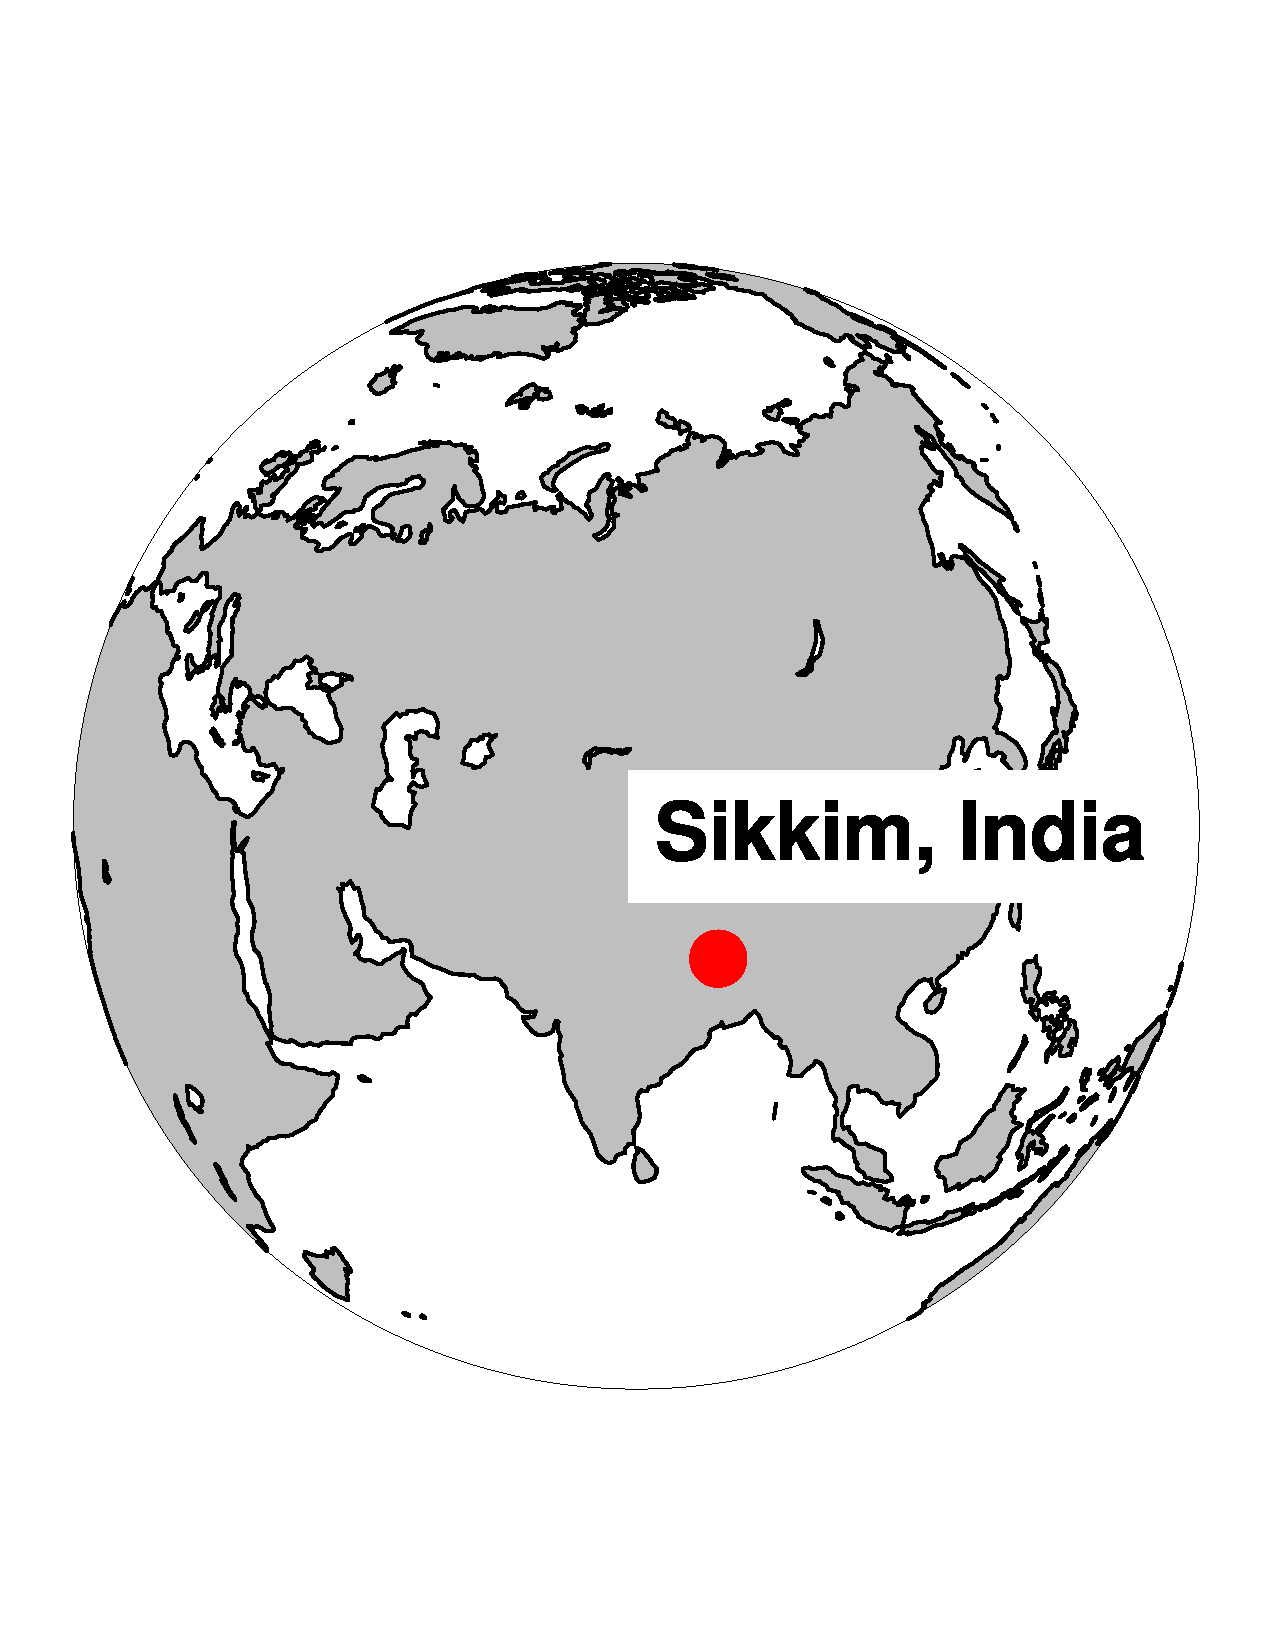
\includegraphics[width=\textwidth]{plot_maxhsurf.pdf}
          \end{minipage}
        \end{tabbing}

        \addtocounter{table}{-1} % we need this because we have a nested table-longtable environment
        \definecolor{bggreen}{cmyk}{0.38, 0.00, 0.25, 0.16 }
        \renewcommand{\baselinestretch}{1.00}\normalsize%
        \pgfkeys{/pgf/number format/set thousands separator={\,}}
        \pgfplotstableread{vertical_half_levels_maxheight_i.txt}{\loadedtable}\vspace*{0pt}%
        \pgfplotstabletypeset[ 
        begin table=\begin{longtable}, 
          end table=\end{longtable},
        columns={k,z,k,z,k,z,k,z},
        every  head row/.style={after row={\hline}},
        precision=2,
        font=\normalsize,
        columns/k/.style={column name=level idx., column type=c, 
          column type/.add={>{\columncolor{bggreen!15}}}{}},
        columns/z/.style={column name=height $[m]$, fixed,dec sep align, zerofill,precision=3},
        display columns/0/.style={select equal part entry of={0}{4},string type},
        display columns/1/.style={select equal part entry of={0}{4}},
        display columns/2/.style={select equal part entry of={1}{4},string type},
        display columns/3/.style={select equal part entry of={1}{4}},
        display columns/4/.style={select equal part entry of={2}{4},string type},
        display columns/5/.style={select equal part entry of={2}{4}},
        display columns/6/.style={select equal part entry of={3}{4},string type},
        display columns/7/.style={select equal part entry of={3}{4}},
        ] {\loadedtable}
      \end{minipage}
    };
  \end{tikzpicture}
\end{table}


\begin{table}[p]
  \caption{Height above ground~$z_i^f(x)$ (full levels) for the grid point with maximum topography height
    in the operational setup R03B07, 13\,km spatial resolution.}
  
  \vspace*{4em}
  \begin{tikzpicture}
    \node[draw,rectangle] (0,0) {
      \begin{minipage}{0.96\textwidth}
        \vspace*{4em}%
        \begin{tabbing}     
          \hspace*{3em}%
          \begin{minipage}[b]{0.55\textwidth}\vspace*{0em}%
            \underline{\textbf{Example: Height above ground, full levels}}\\[1em]
            Location with max.\ surface height\\    
            \begin{tabbing}
              \texttt{CLON}/\texttt{CLAT}   \== 88.180 / 27.938          \\[0.5em]
              \texttt{HSURF}                \>=   6425.974 m
            \end{tabbing}
          \end{minipage}
          \=\hspace*{3em}%
          \begin{minipage}[c]{0.25\textwidth}\vspace*{-8em}%
            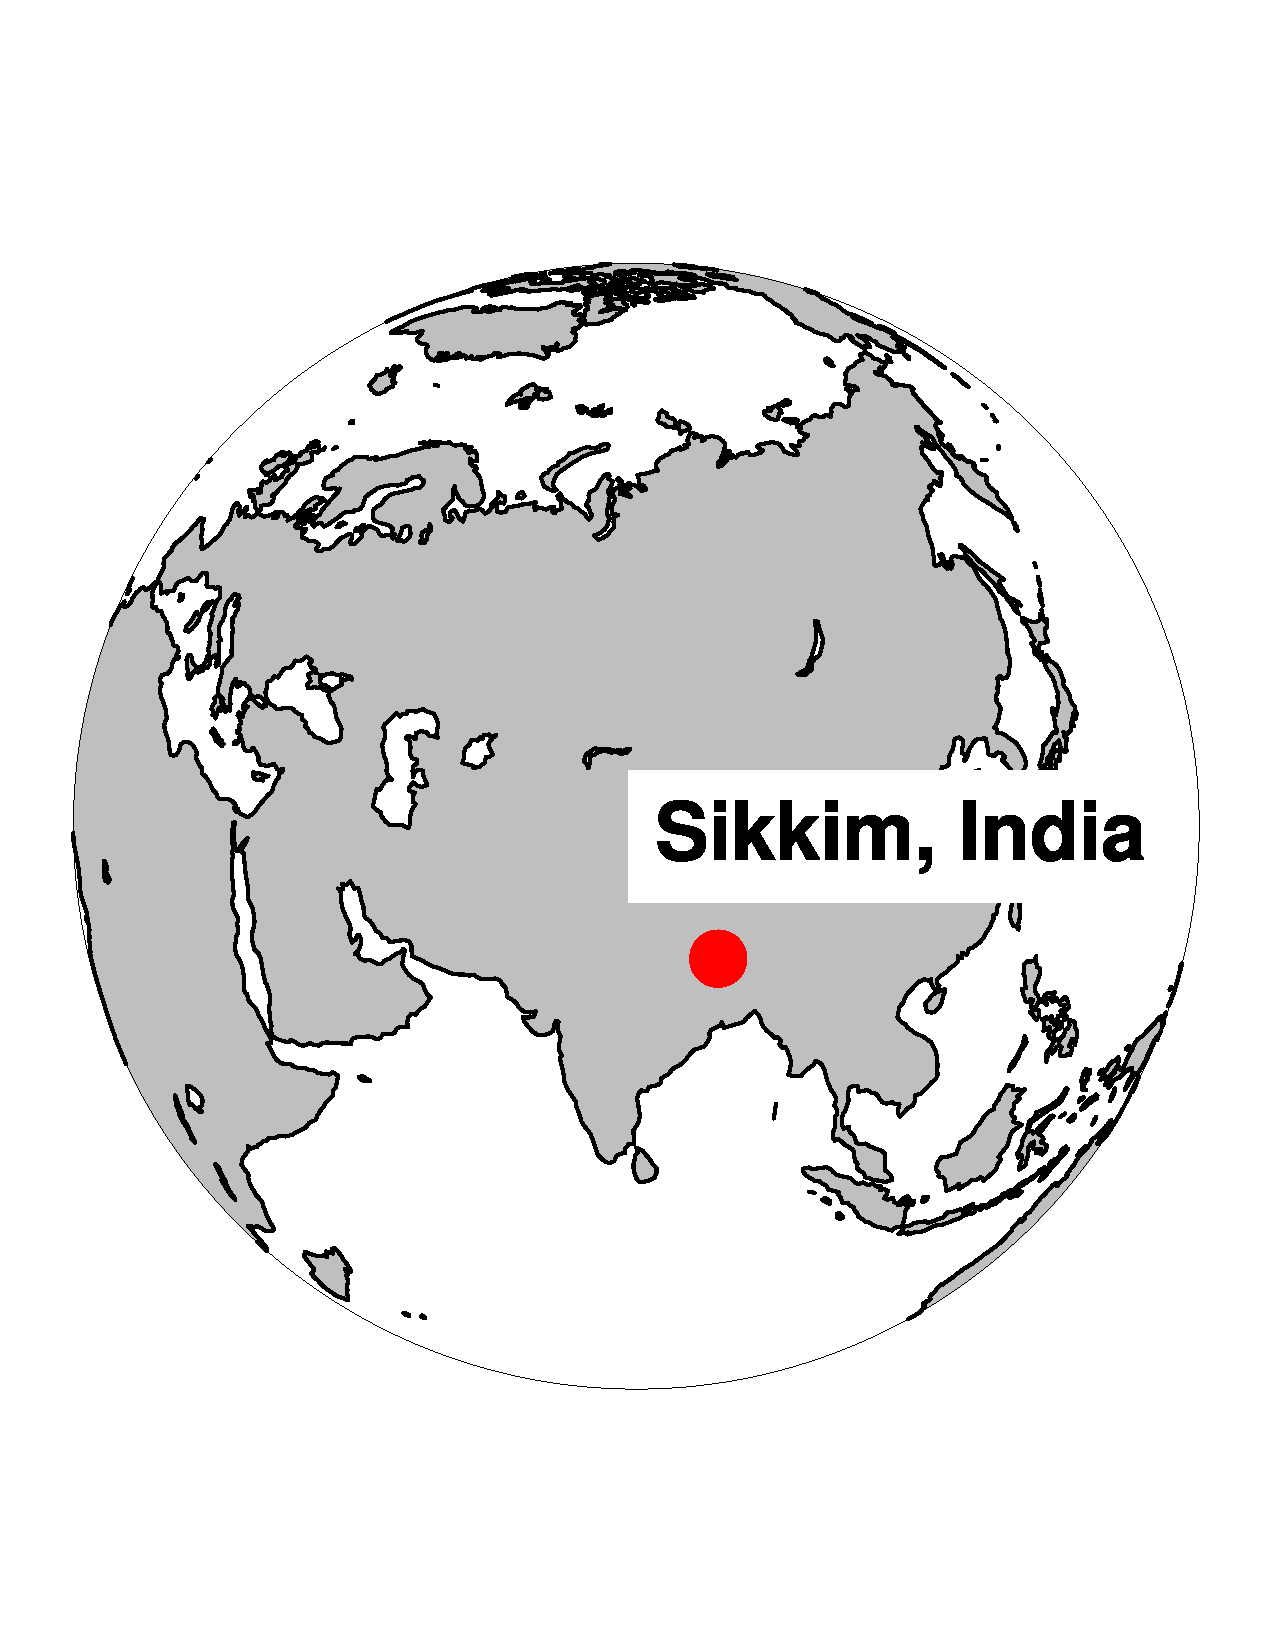
\includegraphics[width=\textwidth]{plot_maxhsurf.pdf}
          \end{minipage}
        \end{tabbing}

        \addtocounter{table}{-1} % we need this because we have a nested table-longtable environment
        \definecolor{bgblue}{cmyk}{ 0.53, 0.20, 0.00, 0.27}
        \renewcommand{\baselinestretch}{1.00}\normalsize%
        \pgfkeys{/pgf/number format/set thousands separator={\,}}
        \pgfplotstableread{vertical_full_levels_maxheight_i.txt}{\loadedtable}\vspace*{0pt}%
        \pgfplotstabletypeset[ 
        begin table=\begin{longtable}, 
          end table=\end{longtable},
        columns={k,z,k,z,k,z,k,z},
        every  head row/.style={after row={\hline}},
        precision=2,
        font=\normalsize,
        columns/k/.style={column name=level idx., column type=c, 
          column type/.add={>{\columncolor{bgblue!15}}}{}},
        columns/z/.style={column name=height $[m]$, fixed,dec sep align, zerofill,precision=3},
        display columns/0/.style={select equal part entry of={0}{4},string type},
        display columns/1/.style={select equal part entry of={0}{4}},
        display columns/2/.style={select equal part entry of={1}{4},string type},
        display columns/3/.style={select equal part entry of={1}{4}},
        display columns/4/.style={select equal part entry of={2}{4},string type},
        display columns/5/.style={select equal part entry of={2}{4}},
        display columns/6/.style={select equal part entry of={3}{4},string type},
        display columns/7/.style={select equal part entry of={3}{4}},
        ] {\loadedtable}
      \end{minipage}
    };
  \end{tikzpicture}
\end{table}  %--- Einbinden der Appendix

% \listoffigures                    %--- Erstellung des Figurenverzeichnisses

% \glsaddall
% \printglossary[type=symbolslist]  %--- Erstellung des Symbolverzeichnisses

% \backmatter
% \bibliography{/home/dreinert/Documents/bibliography/litera.bib,/home/dreinert/Documents/bibliography/litera_notprinted.bib} %--- Erstellen der Liste aller Referenzen
\bibliography{litera.bib} %--- Create list of references

% remove chapter number from header for Acknowledgements
\renewcommand{\chaptermark}[1] {
  \markboth{#1}{}
}
% --- Danksagung ---
% \include{./text/danksagung}

% use default again
\renewcommand{\chaptermark}[1]{%
  \markboth{\chaptername
    \ \thechapter.\ #1}{}}


\end{document}
